\label{key}\documentclass[UTF8,a4paper,11pt]{ctexart}
\usepackage[left=2.50cm, right=2.50cm, top=2.50cm, bottom=2.50cm]{geometry} %页边距
\CTEXsetup[format={\Large\bfseries}]{section} 
 

% compile using Xelatex
%%%%%%%%%%%%%%%%%%%%%%%   字体备选栏
% -- 中文字体 --
%\setmainfont{Microsoft YaHei}  % 微软雅黑
%\setmainfont{YouYuan}  % 幼圆    
%\setmainfont{NSimSun}  % 新宋体
%\setmainfont{KaiTi}    % 楷体
%\setmainfont{SimSun}   % 宋体
%\setmainfont{SimHei}   % 黑体
% -- 英文字体 --
%\usepackage{times}
%\usepackage{mathpazo}
%\usepackage{fourier}
%\usepackage{charter}
\usepackage{helvet}
 
\usepackage{amsmath, amsfonts, amssymb} % math equations, symbols
\usepackage[english]{babel}
\usepackage{color}      % 控制文本颜色
\usepackage{graphicx}   % 加载图像包
\usepackage{url}        % 网址超链接
\usepackage{bm}         % equations的粗体形式
\usepackage{tikz}       % tikz 图像包
\usepackage{multirow}	% 列表设置一格多行多列
\usepackage{ulem}
\usepackage{booktabs}
\usepackage{epstopdf}
\usepackage{epsfig}
\usepackage{algorithm}  %编写算法

\usepackage{hyperref} %此处设置文本内超链接

%\usepackage{CJK,pgf,pgfarrows,pgfnodes,pgfautomata,pgfheaps}
\usepackage{amsmath,amssymb}
\usepackage{geometry}%页面设置
\usepackage{graphicx}%图片设置
\usepackage{float} %指定图片位置
%\usepackage{subfig}%多个子图
\usepackage{subfigure}%并排子图 共享标题 有子标题
\usepackage{caption}%注释设置

\usepackage{algorithm}
\usepackage{algorithmicx}
\usepackage{algpseudocode}  

% 这个和algorithmic不兼容,用了就要报错,好多莫名其妙的错误!!!!!
\floatname{algorithm}{算法}  
\renewcommand{\algorithmicrequire}{\textbf{输入:}}  
\renewcommand{\algorithmicensure}{\textbf{输出:}}  
\renewcommand{\algorithmicrequire}{ \textbf{Input:}}     %Use Input in the format of Algorithm
\renewcommand{\algorithmicensure}{ \textbf{Output:}}    %UseOutput in the format of Algorithm

\newtheorem{pf}{Pf}
\newtheorem{sol}{Sol}[section]
\newtheorem{thm}{Thm}
% 算法示例备选项
%\renewcommand{\algorithmicrequire}{ \textbf{Input:}}     % use Input in the format of Algorithm  
%\renewcommand{\algorithmicensure}{ \textbf{Initialize:}} % use Initialize in the format of Algorithm  
%\renewcommand{\algorithmicreturn}{ \textbf{Output:}}     % use Output in the format of Algorithm  

\DeclareMathOperator{\dif}{d\!}  %定义微分的缩写
\DeclareMathOperator{\pa}{\partial}  %定义偏微分的缩写

%\usepackage{fancyhdr}  %这里对 页眉、页脚 进行设置
%\pagestyle{fancy}
%\rhead{\thepage}
%\chead{}
%%\lhead{\includegraphics[width=1.6cm]{wallpaper.jpg}}
%\lfoot{}
%\cfoot{Page \thepage{} of \pageref{LastPage}}
%\rfoot{}
%
%\newcommand{\makeheadrule}{%        %去除页眉的横线 以免遮挡后面文字 
%	\makebox[0pt][l]{\rule[0\baselineskip]{\headwidth}{0pt}}%
%	\rule[0\baselineskip]{\headwidth}{0pt}}
%\renewcommand{\headrule}{%
%	{\if@fancyplain\let\headrulewidth\plainheadrulewidth\fi
%		\makeheadrule}}

%\usepackage[printwatermark]{xwatermark}   %%这以下设置“数学外卖”官方水印
%\usepackage{lipsum}
%
%\newsavebox\mybox
%
%\savebox\mybox{\tikz[color=gray,opacity=0.3]
%\newwatermark*[
%allpages,
%angle=48,
%scale=6,
%xpos=-20,
%ypos=15
%]{\usebox\mybox} 
 


\title{\textbf{Homework 7}}
\author{ 张思源  \qquad  \textit{21110850018} }   %这里填上您的大名


\begin{document}
\maketitle
\section{Ex1}
\begin{sol}
	首先导入数据,将列名更改为特征名称,并打印前$5$行可以得到结果如下图:
	\begin{figure}[H]
		\centering
		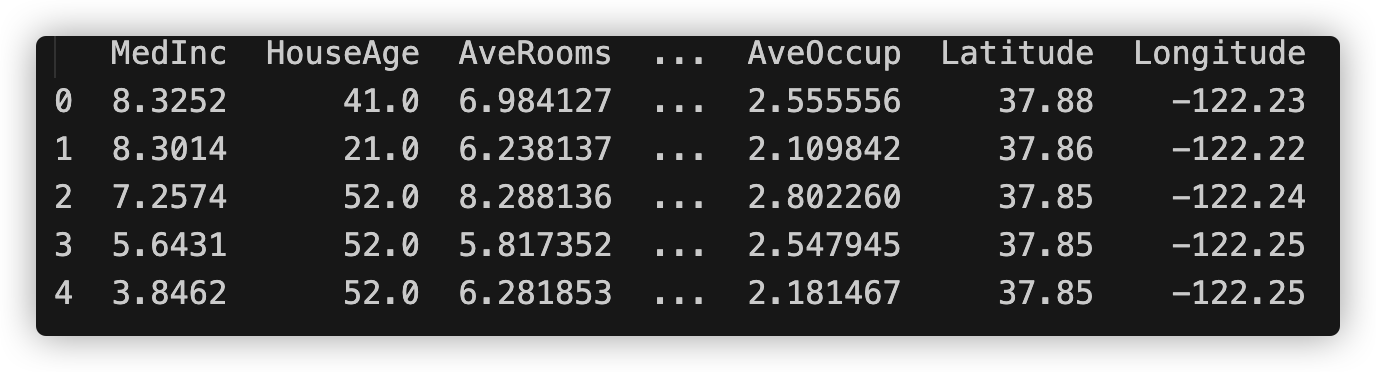
\includegraphics[width=0.95\textwidth,height=0.6\textwidth]{head.png}
		\caption{Head of the data}
	\end{figure}
	然后,打印房价(即target)的最值,可以发现其最大值为$5.00001$,最小值为$0.14999$.
	进而计算模型的VIF(方差膨胀系数):可以得到$8$个特征的VIF系数依次为:
	$11.51$,$7.20$,$45.99$,
	$43.59$,$2.94$,$1.10$, 
	$559.87$,$633.71$,可以看出第1个、第3个、第4个特征的VIF系数超过了$10$,第7个和第8个
	特征的VIF系数更是超过了$100$,说明数据存在多重共线性.\\

	对数据集分别利用多元线性回归、岭回归和Lasso回归模型,可以得到模型的$MSE$和
	$adjustR^{2}$分别如下图所示,其中
	$$adjustR^{2}=1-\frac{(1-R^{2})(n-1)}{n-p-1}$$
	\begin{figure}[H]
		\centering
		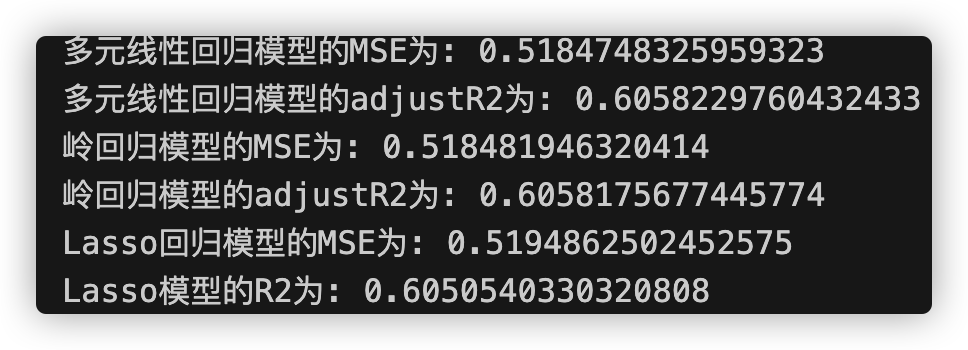
\includegraphics[width=0.95\textwidth,height=0.6\textwidth]{model.png}
		\caption{$MSE$ and $adjustR^{2}$ of 3 models}
	\end{figure}
	最后,比较不同的正则化项可得下表:
	\begin{center}
		\begin{tabular}{c p{5cm} p{5cm}}
		
		\hline
		 & Lasso(L1正则项) & Ridge(L2正则项) \\
		\hline
		相同点 &都可以用来解决过拟合问题  \\
		不同点 & 可以用来做 feature selection,更容易使得权重变为0 & 不可以做 feature selection,更容易使得权重接近0\\
		\hline
	\end{tabular}
	\end{center}
\section{Ex2}
\begin{sol}
	首先,计算得:
	\begin{equation*}
		\begin{split}
			\frac{\partial E}{\partial w_{kj}}&=\frac{\partial E}{\partial o_{k}} \frac{\partial o_{k}}{\partial net_{k}} \frac{\partial net_{k}}{\partial w_{kj}}\\
			&=(o_{k}-d_{k})f(\sum_{j=0}^{m}w_{kj}y_{j})(1-(\sum_{j=0}^{m}w_{kj}y_{j}))y_{j}\\
			&=(o_{k}-d_{k})o_{k}(1-o_{k})y_{j}
		\end{split}
	\end{equation*}
	所以$\Delta w_{kj}=-\eta (o_{k}-d_{k})o_{k}(1-o_{k})y_{j}$.并且可以计算得:
	\begin{equation*}
		\begin{split}
			\frac{\partial E}{\partial v_{ji}}&=\sum_{k=1}^{l}\frac{\partial E}{\partial o_{k}} \frac{\partial o_{k}}{\partial net_{k}} \frac{\partial net_{k}}{\partial y_{j}} \frac{\partial y_{j}}{\partial net_{j}} \frac{\partial net_{j}}{\partial v_{ji}}\\
			&=\sum_{k=1}^{l}(o_{k}-d_{k})f(\sum_{j=0}^{m}w_{kj}y_{j})(1-f(\sum_{j=0}^{m}w_{kj}y_{j}))w_{kj}f(\sum_{i=0}^{n}v_{ji}x_{i})(1-f(\sum_{i=0}^{n}v_{ji}x_{i}))x_{i}\\
			&=\sum_{k=1}^{l}(o_{k}-d_{k})o_{k}(1-o_{k})w_{kj}y_{j}(1-y_{j})x_{i}
		\end{split}
	\end{equation*}
	所以$\Delta v_{ji}=-\eta \sum_{k=1}^{l}(o_{k}-d_{k})o_{k}(1-o_{k})w_{kj}y_{j}(1-y_{j})x_{i}$.
\end{sol}

\end{sol}






\newpage
\begin{thebibliography}{3}  
	\bibitem{ref1} 李航. 统计学习方法[M]. 清华大学出版社, 2012.
	%\bibitem{ref2} Kingma D , Ba J . Adam: A Method for Stochastic Optimization[J]. Computer Science, %2014.
	\bibitem{ref2} Goodfellow, Ian, et al. Deep Learning[M]. MIT Press, 2016. 	
\end{thebibliography}
\end{document}
